\documentclass[11pt]{article}
\usepackage[a4paper, top=2.5cm, bottom=2.5cm, left=2.5cm, right=2.5cm]{geometry}
\usepackage{amsmath, amssymb}
\usepackage{xcolor}
\usepackage{graphicx}
\newsavebox{\dtxbox}
\usepackage{tikz}
\usetikzlibrary{cd}
\makeatletter % quantikz2 restyles every tikz-cd diagram: keep tikz-cd's own look outside quantum circuits
\pgfkeysgetvalue{/tikz/commutative diagrams/every cell/.@cmd}\dtx@cdcell
\pgfkeysgetvalue{/tikz/commutative diagrams/arrows/.@cmd}\dtx@cdarrows
\pgfkeysgetvalue{/tikz/commutative diagrams/row sep/normal}\dtx@cdrow
\pgfkeysgetvalue{/tikz/commutative diagrams/column sep/normal}\dtx@cdcol
\newcommand\dtx@cdplain{%
  \pgfkeyslet{/tikz/commutative diagrams/every cell/.@cmd}\dtx@cdcell
  \pgfkeyslet{/tikz/commutative diagrams/arrows/.@cmd}\dtx@cdarrows
  \pgfkeyslet{/tikz/commutative diagrams/row sep/normal}\dtx@cdrow
  \pgfkeyslet{/tikz/commutative diagrams/column sep/normal}\dtx@cdcol
  \tikzset{nodes in empty cells=false}%
  \let\DivideRowsCols\relax}
\AddToHook{env/tikzcd/begin}{\dtx@cdplain}
\makeatother
\usetikzlibrary{arrows.meta, decorations.pathmorphing, quantikz2}
\usepackage{pgfplots}
\pgfplotsset{compat=1.18}
\usepackage{circuitikz}
\usepackage{tikz-cd}
\definecolor{tdc1}{HTML}{6B6B6B}
\definecolor{tdc2}{HTML}{E8F0FB}
\definecolor{tdc3}{HTML}{E6F4EA}
\definecolor{tdc4}{HTML}{A05A5A}
\definecolor{tdc5}{HTML}{1E5BD6}
\definecolor{tdc6}{HTML}{D62728}
\definecolor{tdc7}{HTML}{1E63C4}

\title{Welcome to DiagramTeX}
\date{}

\begin{document}
\maketitle

\begin{center}
\begin{lrbox}{\dtxbox}%
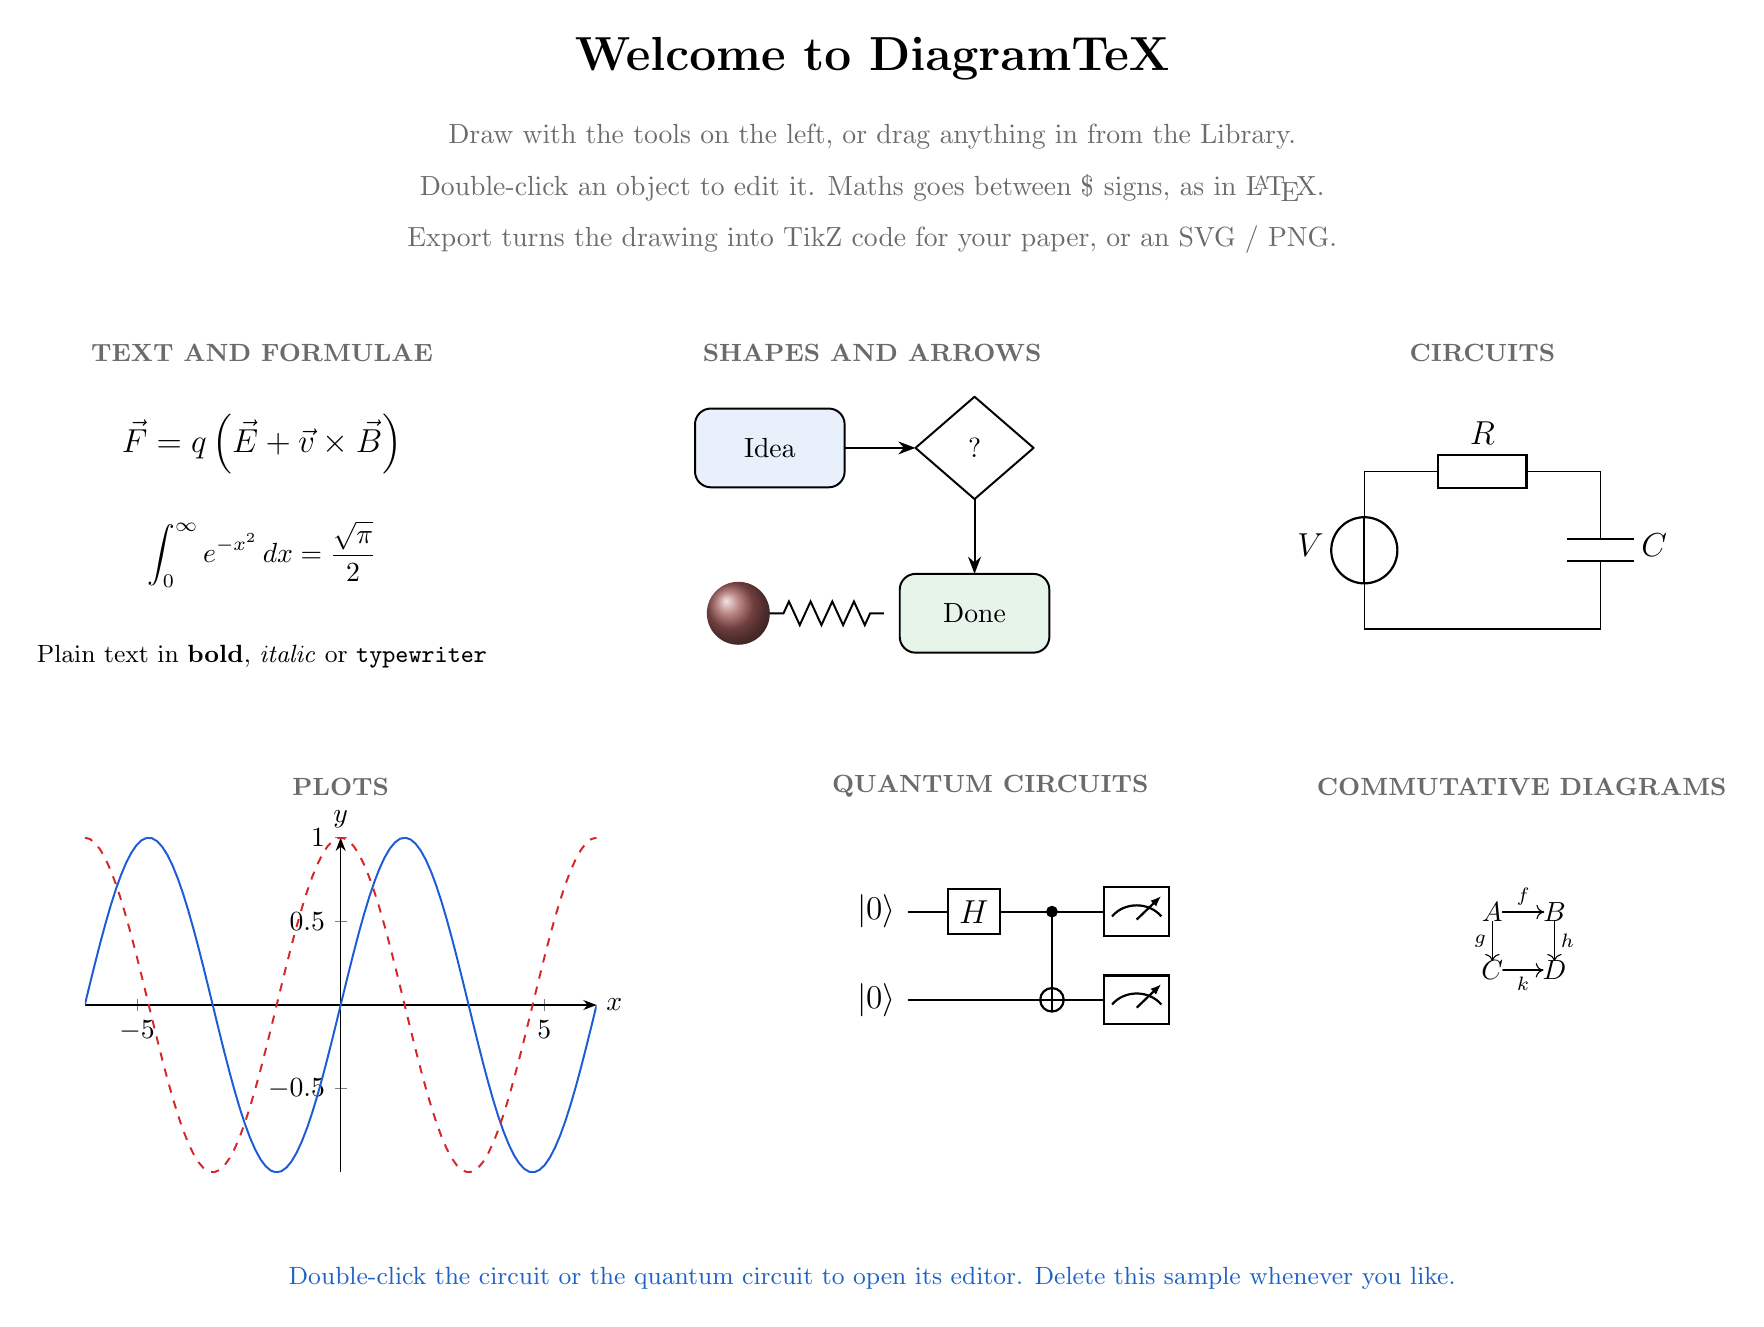
\begin{tikzpicture}[x=1cm, y=1cm]
  \node[font=\LARGE\bfseries] at (11,0) {Welcome to DiagramTeX};
  \node[text=tdc1] at (11,-1) {Draw with the tools on the left, or drag anything in from the Library.};
  \node[text=tdc1] at (11,-1.65) {Double-click an object to edit it. Maths goes between \textdollar\ signs, as in \LaTeX.};
  \node[text=tdc1] at (11,-2.3) {Export turns the drawing into TikZ code for your paper, or an SVG / PNG.};
  \node[font=\small\bfseries, text=tdc1] at (3.25,-3.75) {TEXT AND FORMULAE};
  \node[font=\large] at (3.25,-4.9) {$\vec F = q\left(\vec E + \vec v \times \vec B\right)$};
  \node at (3.25,-6.3) {$\displaystyle\int_0^\infty e^{-x^2}\,dx = \frac{\sqrt{\pi}}{2}$};
  \node[font=\small] at (3.25,-7.6) {Plain text in \textbf{bold}, \textit{italic} or \texttt{typewriter}};
  \node[font=\small\bfseries, text=tdc1] at (11,-3.75) {SHAPES AND ARROWS};
  \draw[line width=0.71pt, fill=tdc2, line join=round] (8.95,-4.45) -- (10.45,-4.45) -- (10.45,-4.45) .. controls (10.56,-4.45) and (10.65,-4.54) .. (10.65,-4.65) -- (10.65,-5.25) -- (10.65,-5.25) .. controls (10.65,-5.36) and (10.56,-5.45) .. (10.45,-5.45) -- (8.95,-5.45) -- (8.95,-5.45) .. controls (8.84,-5.45) and (8.75,-5.36) .. (8.75,-5.25) -- (8.75,-4.65) -- (8.75,-4.65) .. controls (8.75,-4.54) and (8.84,-4.45) .. (8.95,-4.45) -- cycle;
  \node[align=center] at (9.7,-4.95) {Idea};
  \draw[line width=0.71pt, -{Stealth}] (10.65,-4.95) -- (11.55,-4.95);
  \draw[line width=0.71pt, line join=round] (12.3,-4.3) -- (13.05,-4.95) -- (12.3,-5.6) -- (11.55,-4.95) -- cycle;
  \node[align=center] at (12.3,-4.95) {$?$};
  \draw[line width=0.71pt, -{Stealth}] (12.3,-5.6) -- (12.3,-6.55);
  \draw[line width=0.71pt, fill=tdc3, line join=round] (11.55,-6.55) -- (13.05,-6.55) -- (13.05,-6.55) .. controls (13.16,-6.55) and (13.25,-6.64) .. (13.25,-6.75) -- (13.25,-7.35) -- (13.25,-7.35) .. controls (13.25,-7.46) and (13.16,-7.55) .. (13.05,-7.55) -- (11.55,-7.55) -- (11.55,-7.55) .. controls (11.44,-7.55) and (11.35,-7.46) .. (11.35,-7.35) -- (11.35,-6.75) -- (11.35,-6.75) .. controls (11.35,-6.64) and (11.44,-6.55) .. (11.55,-6.55) -- cycle;
  \node[align=center] at (12.3,-7.05) {Done};
  \shade[ball color=tdc4] (9.3,-7.05) circle (0.4);
  \draw[line width=0.71pt, decorate, decoration={zigzag, segment length=0.2752cm, amplitude=0.15cm, pre length=0.174cm, post length=0.174cm}] (9.7,-7.05) -- (11.15,-7.05);
  \node[font=\small\bfseries, text=tdc1] at (18.75,-3.75) {CIRCUITS};
  \begin{scope}[shift={(17.25,-7.25)}, font=\large]
    \draw (0,0) to[european voltage source, l=$V$] (0,2);
    \draw (0,2) to[european resistor, l=$R$] (3,2);
    \draw (3,2) to[capacitor, l=$C$] (3,0);
    \draw (3,0) -- (0,0);
  \end{scope}
  \node[font=\small\bfseries, text=tdc1] at (4.25,-9.25) {PLOTS};
  \begin{axis}[
    at={(1cm,-14.15cm)},
    anchor=south west,
    scale only axis,
    width=6.5cm,
    height=4.25cm,
    xmin=-6.2832,
    xmax=6.2832,
    ymin=-0.9999,
    ymax=1,
    xtick={-5,0,5},
    ytick={-0.5,0,0.5,1},
    axis lines=middle,
    axis line style={-{Stealth}},
    every axis x label/.style={at={(current axis.right of origin)}, anchor=west},
    every axis y label/.style={at={(current axis.above origin)}, anchor=south},
    xlabel={$x$},
    ylabel={$y$}
  ]
    \addplot[color=tdc5, line width=0.71pt, no marks, domain=-6.2832:6.2832, samples=100, forget plot] {sin(deg(x))};
    \addplot[color=tdc6, line width=0.71pt, dashed, no marks, domain=-6.2832:6.2832, samples=100, forget plot] {cos(deg(x))};
  \end{axis}
  \node[font=\small\bfseries, text=tdc1] at (12.5,-9.25) {QUANTUM CIRCUITS};
  \node[font=\large] at (12.79,-11.32) {\pgfinterruptpicture%
  \begin{quantikz}
  \lstick{\ket{0}} & \gate{H} & \ctrl{1} & \meter{} \\
  \lstick{\ket{0}} & & \targ{} & \meter{}
  \end{quantikz}%
  \endpgfinterruptpicture};
  \node[font=\small\bfseries, text=tdc1] at (19.25,-9.25) {COMMUTATIVE DIAGRAMS};
  \node at (19.28,-11.19) {\pgfinterruptpicture%
  \begin{tikzcd}
    A \arrow[r, "f"] \arrow[d, "g"'] & B \arrow[d, "h"] \\
    C \arrow[r, "k"']                  & D
  \end{tikzcd}%
  \endpgfinterruptpicture};
  \node[font=\small, text=tdc7] at (11,-15.5) {Double-click the circuit or the quantum circuit to open its editor. Delete this sample whenever you like.};
\end{tikzpicture}
\end{lrbox}%
\resizebox{\linewidth}{!}{\usebox{\dtxbox}}
\end{center}

\end{document}
